\subsubsection{Prototyp}
\label{sec:Prototyp}

Nach Bereitstellung des Ticketsystems und des Versionierungstools kann mit der Implementierung der Software begonnen werden. Für die Auftraggeber des Projektes war es dabei besonders wichtig, dass zunächst ein Prototyp der späteren Software entwickelt wird. Dieser Prototyp sollte nur die 360 Grad Ansicht eines Campus Panoramas und die Möglichkeit zu einem weiteren Panorama zu navigieren enthalten. Der Prototyp sollte genutzt werden um Entscheidungsträger von Beginn an vom Projekt zu überzeugen.

Da der Prototyp nur einen statischen Einblick (kein dynamischer Inhalt aus einer Datenbank) in die späteren Benutzeransicht gewähren sollte, wurde hierfür ein HTML-Dokument geschrieben, das die Google Street View API einbindet und über Javascript dessen Funktionalität implementiert. Das erstellte HTML-Dokument ist in \listing{HTML Prototyp} dargestellt:

\lstinputlisting[language=HTML,caption={HTML Prototyp},label={lst:HTML Prototyp}]{Listings/HTML_Prototyp.html}

Das dargestellte HTML-Dokument bindet in Zeile 5 die angesprochene Google Street View API, in der Funktionen zur Darstellung des 360 Grad Panoramas definiert sind. Zusätzlich wird in Zeile 6 eine Javascript-Datei eingebunden, in der die Funktionen der Google Street View API auferufen werden. Im Body-Bereich des HTML-Dokumentes ist dafür ein Element definiert das als Fläche zur Darstellung der Panoramas genutzt wird. Die eingebundene Javascript-Datei aus Zeile 6 ist aus Platzgründen in \listing{Javascript Prototyp} in Anhang ~\ref{sec:AnhangJavascriptPrototyp} dargestellt. Dessen Funktionalität wird an dieser Stelle kurz erläutert.

Sobald der Internetbrowser des Benutzers das HTML-Dokument fertig geladen hat, wird eine Methode aufgerufen, die benötigte Parameter zur Erstellung des Panoramas bereitstellt\footnote{Vergleiche Zeile 3 im Anhang XX}. Hier werden Zoomstufe, Ausrichtung und weitere Parameter festgelegt. Anschließend wird ein Panorama-Objekt mit Hilfe der Google Street View API erstellt und an das oben beschriebene HTML-Element im Body-Bereich gebunden\footnote{Vergleiche Zeile 16-18 im Anhang XX}. Über einen weiteren Aufruf einer API-Funktion können an das Panorama sogenannte "`Links"' gehängt werden. Diese Links stellen später für den Benutzer die Pfeile am Boden dar über die zu anderen Panoramas navigiert werden kann. Im Prototyp wird nur der Verweis auf ein anderes Panorama gebraucht, das über die Funktion "`createCustomLinks"'\footnote{vergleiche Zeile 45ff. im Anhang XX} als Link angehängt wird.

Ein Bildschirmfoto des Prototypen der mit diesen zwei Dateien (HTML- und Javascript-Dokument) erstellt wurde ist in \abbildung{PrototypScreenshot} zu sehen.

%TODO: Screenshot ohne Pixelfehler machen!
\begin{figure}[htb]
\centering
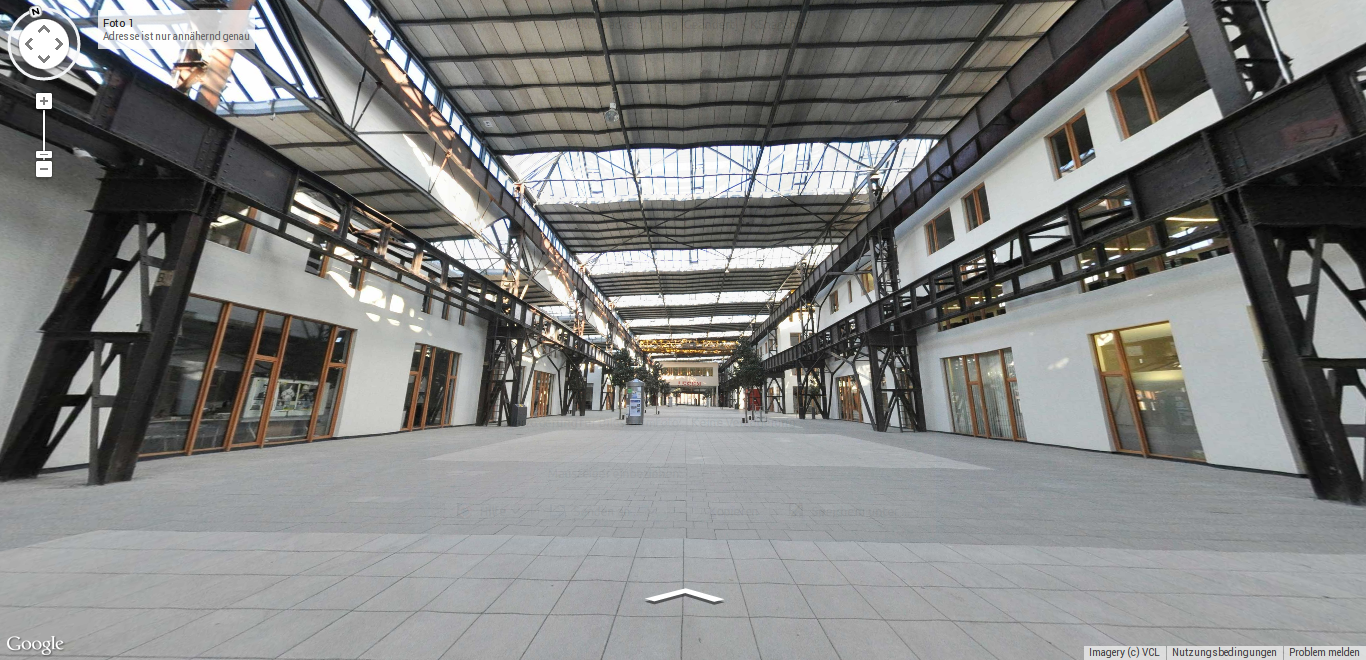
\includegraphics[width=1.0\textwidth]{PrototypScreenshot.png}
\caption[PrototypScreenshot]{Bildschirmfoto des Prototypen}
\label{fig:PrototypScreenshot}
\end{figure}